\section{Обзор литературы}

\subsection{Рентгеновская кристаллография}


Рентгеновская кристаллография является важнейшим инструментом определения трехмерных структур кристаллов. Этот метод позволяет получить бесценные сведения об атомных и молекулярных структурах кристаллов, что крайне важно для понимания свойств и функций материалов в различных областях, включая химию, биологию и материаловедение. Рентгеноструктурный анализ основан на упругом рассеянии монохроматического рентгеновского излучения на трехмерной регулярной решетке атомов твердого вещества, что приводит к интерференции рентгеновских лучей.

\begin{figure}[H]
	\centering
	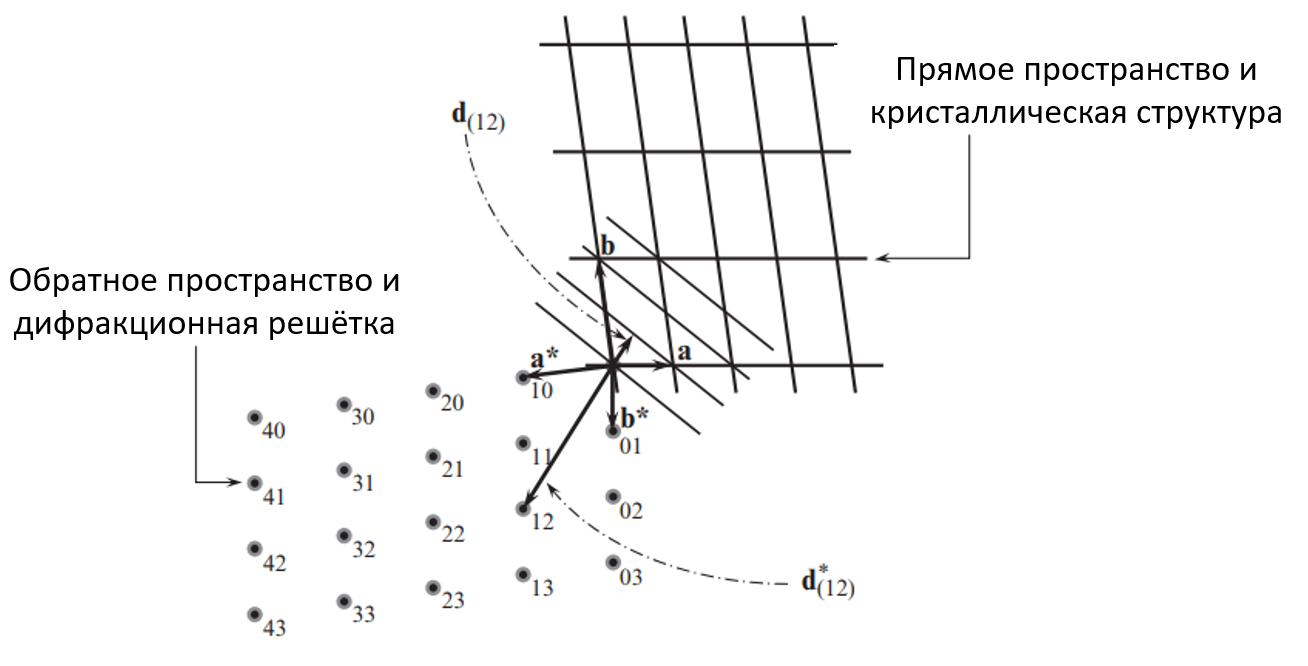
\includegraphics[width=0.8\textwidth]{figures/direct_reciprocal.png}\hfill
	\caption{Связь прямого и обратного пространства \cite{girolami_x-ray_2016}}
	\label{hkl}
\end{figure}

Дифракция в кристалле описывается как отражения от семейств параллельных кристаллографических плоскостей элементарной ячейки кристалла (рис. \ref{hkl}). Каждая точка дифракционной картины задается набором из индексов Миллера $h,k,l$. Угол отражения (рассеяния) $\Theta$ для дифракционного максимума с межплоскостным расстоянием d$_{hkl}$, полученного при рассеянии рентгеновского излучения с длиной волны $\lambda$, определяется из закона Вульфа--Брэгга (уравнение \ref{wb}). Также вводится обратное пространство, где каждая точка задаёт семейства кристаллографических плоскостей структуры, а значит, и отражения. Вместо индексов Миллера можно ввести вектор обратного пространства, задающий отражение $\overrightarrow{H} = (h,k,l)$. Таким образом, дифракционная картина кристалла является трансформацией упорядоченной атомной структуры в обратное пространство.

\begin{equation}\label{wb}
	\mathrm{2d_{hkl}\sin\Theta = \lambda,}
\end{equation}

Любой дифракционный максимум также имеет математическое описание его интенсивности, известное как структурный фактор $F(\overrightarrow{H})$, зависящий от расположения $r_j = (x,y,z)$ и коэффициентов рассеяния $f_j$ всех атомов в элементарной ячейке кристалла:

\begin{equation}\label{eq1}
	\mathrm{ 
		F(\overrightarrow{H}) = |F(\overrightarrow{H})|\exp(i\phi) = \sum\limits_{j=1}^N F_j (\overrightarrow{H}) = \sum\limits_{j=1}^N f_j \exp(2\pi i(\overrightarrow{H},\overrightarrow{r_j}))),}
\end{equation}

где $(\overrightarrow{H}, \overrightarrow{r_j}) = hx_j+ky_j+lz_j$, F$_j$ --- структурный фактор каждого из N симметрично независимых атомов в кристаллической ячейке, в котором закодирована информация об амплитуде f$_j$ и фазе $\phi_j = 2\pi (\overrightarrow{H}, \overrightarrow{r_j})$ рассеяной этим атомом волны.



\subsection{Проблема фаз}

Структурный фактор, как следует из определения (уравнение \ref{eq1}), является комплексной величиной, которая описывает вклад дифракции всех атомов кристаллической решетки в отражение. Стоит отметить, что оно было получено в следующем приближении:

\begin{itemize}
\item Элементарная ячейка поделена на $N$ атомов в точках $\overrightarrow{r_j}$.

\item Каждый из атомов рассеивает волну с амплитудой $f_j$  и фазой $\phi_j = 2\pi (\overrightarrow{H}, \overrightarrow{r_j})$.
\end{itemize}

Перейдем к более общему описанию --- заменим атомы на маленькие параллелепипеды, внутри которых находятся электроны и рассеивают излучение. Тогда предыдущее приближение превращается в следующее:

\begin{itemize}
\item Элементарная ячейка поделена на $N$ маленьких параллелепипедов, объем каждого $\Delta V$ и позиция $\overrightarrow{r_j}$.

\item Каждый из параллелепипедов рассеивает волну с амплитудой $\rho(\overrightarrow{r_j})\Delta V$  и фазой $\phi_j = 2\pi (\overrightarrow{H}\cdot\overrightarrow{r_j})$, где $\rho(\overrightarrow{r_j})$ --- электронная плотность внутри параллелепипеда.
\end{itemize}

Тогда выражение \ref{eq1} можно записать следующим образом, устремив объемы параллелепипедов к нулю:

\begin{equation}\label{eq2}
\mathrm{ 
F(h,k,l) = \sum\limits_{j=1}^N \rho(\overrightarrow{r_j})\Delta V_j \exp(2\pi i(\overrightarrow{H}\cdot\overrightarrow{r_j})) = \int_V\rho(\overrightarrow{r})\exp(2\pi i(\overrightarrow{H}\cdot\overrightarrow{r_j}))dV,}
\end{equation}

где интегрирование ведется по всему объему элементарной ячейки.

Можно заметить, что уравнение \ref{eq2} является обратным преобразованием Фурье, переводящее электронную плотность в структурные факторы. Тогда можно записать прямое преобразование Фурье:

\begin{equation}\label{eq21}
\mathrm{ 
\rho(\overrightarrow{r}) = \int F(\overrightarrow{H}) \exp (-2\pi i (\overrightarrow{H}\cdot\overrightarrow{r}))dV^* = \frac{1}{V} \sum\limits_{\overrightarrow{H}} F(\overrightarrow{H}) \exp(-2\pi i (\overrightarrow{H}\cdot\overrightarrow{r_j}))},
\end{equation}

где интегрирование ведётся по обратной ячейке.

\begin{figure}[H]
	\centering
	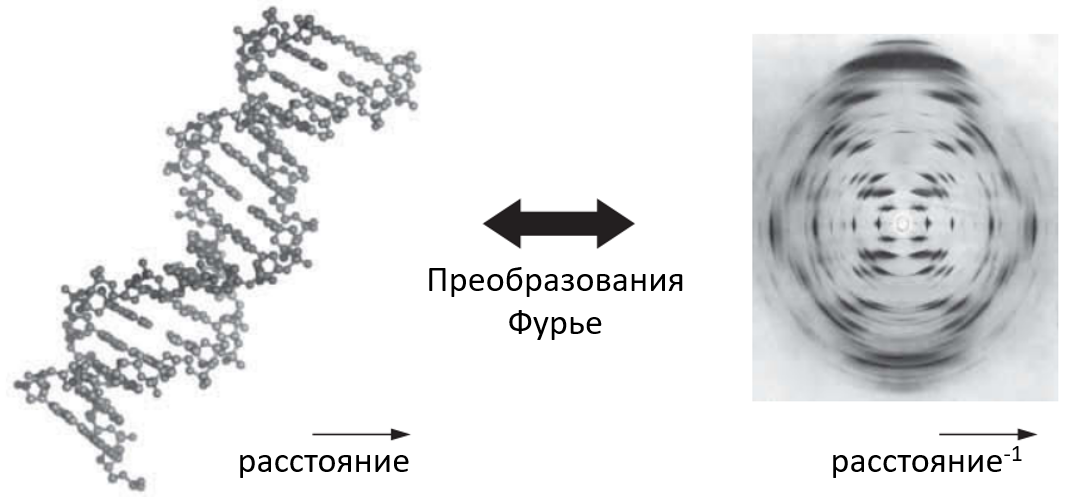
\includegraphics[width=0.8\textwidth]{figures/furie.png}\hfill
	\caption{Схема связи электронной плотности и структурных факторов \cite{girolami_x-ray_2016}}
	\label{furie}
\end{figure}


Если амплитуда и фазы всех дифрагированных лучей были бы зарегистрированы, можно было бы рассчитать распределение электронной плотности в кристалле, применив преобразвование Фурье к дифракционной картине (рис. \ref{furie}). Однако в ходе рентгенодифракционного эксперимента регистрируется лишь интенсивность излучения, информация о фазах теряется, и для получения кристаллической структуры требуется решить так называемую "проблему фаз" или "фазовую проблему".

Таким образом, в идеальном случае, при сохранении полной информации о фазах в ходе эксперимента, структура кристалла могла бы быть непосредственно восстановлена из измеренных амплитуд с помощью преобразования Фурье. Поскольку же фазовая составляющая оказывается неизвестной при рентгеновском рассеянии, расчет электронной плотности становится принципиально затруднённым. Эта утрата фазовой информации, известная как фазовая проблема, представляет собой центральную проблему рентгеновской кристаллографии, и в последующих разделах будут рассмотрены основные методы её решения.


\begin{figure}[H]
	\centering
	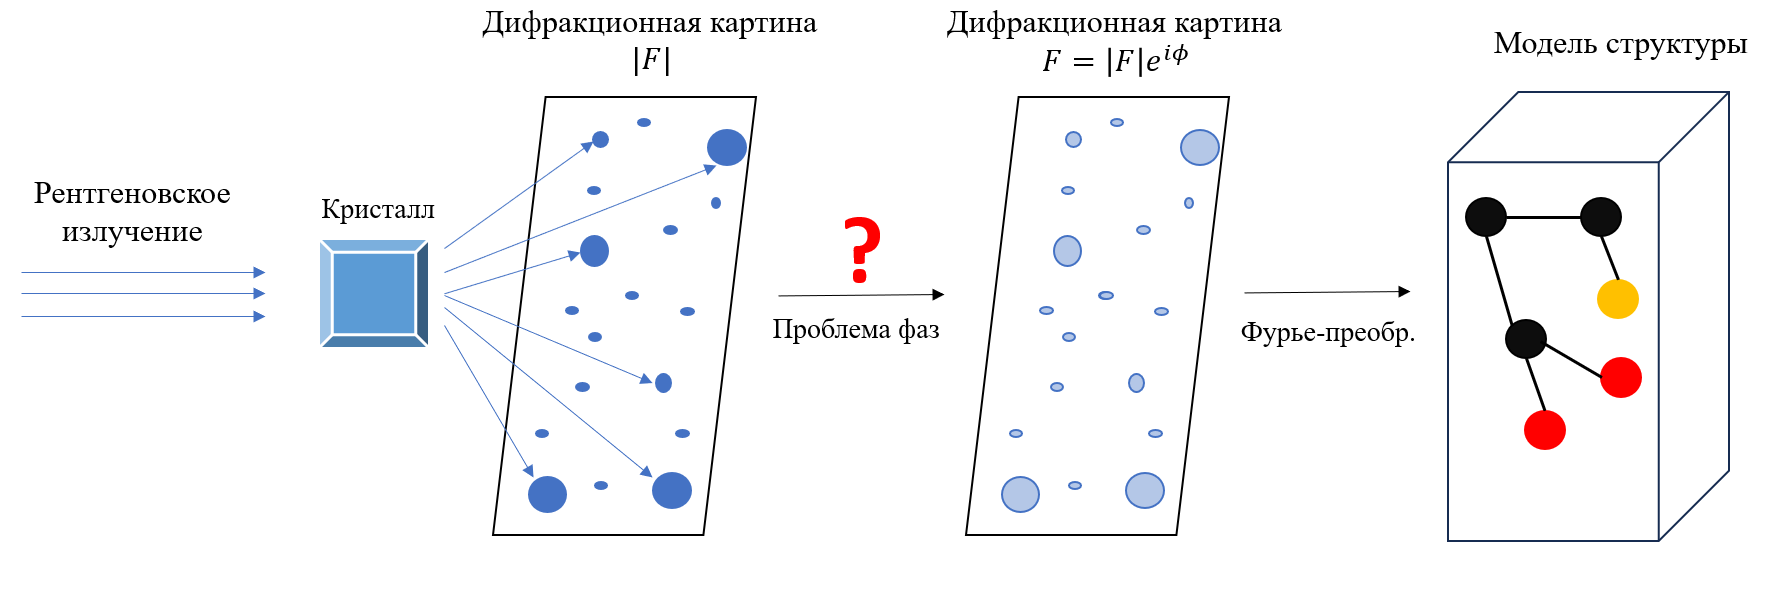
\includegraphics[width=1.0\textwidth]{figures/determination.png}\hfill
	\caption{Cхема определения кристаллической структуры}
	\label{determination}
\end{figure}


\subsection{Решение фазовой проблемы}

\subsubsection{Методы проб и ошибок}

В 1913 году физиком Уильямом Генри Брэггом и его сыном Уильямом Лоренсом Брэггом, были впервые описаны структуры таких веществ, как NaCl, KCl, KBr и KI, с помощью дифракции рентгеновских лучей на кристаллах \cite{hauptman_phase_1951}. Для расшифровки структур тогда использовали так называемые методы проб и ошибок (trial-and-error), которые основаны на достаточно простой идее. Вместо того, чтобы анализировать дифракционную картину, ученые предполагали структуру из известной информации о веществе. Методы проб и ошибок могут использовать следующую информацию для формирования модели структуры: возможные пространственные группы симметрии, число формульных единиц в элементарной ячейке $Z$, симметрия молекулы, структуры подобных кристаллов и соединений, а также физические свойства кристалла. После этого рассчитывали структурные факторы и интенсивности с помощью обратного преобразования Фурье (уравнение \ref{eq2}) и сравнивали полученный набор отражений с экспериментальным. Если наборы данных соответствуют друг другу, то предполагаемую структуру можно считать похожей на истинную и уточнить её, изменяя параметры, пока не будет достаточное совпадение с наблюдаемой дифракционной картиной. В ином случае предположение отвергалось и проверялась другая структура.

Несмотря на кажущуюся простоту, методы проб и ошибок актуальны по сей день. Так, методы молекулярного и изоморфного замещения являются одними из основных способов определения структур белковых соединений, поскольку их кристаллы слабо рассеивают и полученного набора рентгенодифракционных максимумов недостаточно для решения методами, эффективными для низкомолекулярных соединений \cite{lattman_protein_2008-1}, \cite{margiolaki_powder_2008}. Основаны они на дополнительном знании о структурах белков с той же аминокислотной последовательностью (молекулярное замещение) или результатах дифракционных экспериментов структуры того же белка с тяжелыми атомами (изоморфное замещение). Информация используется для построения начальной структуры, которая затем подбирается и уточняется.

Также нельзя не упомянуть важный  результат эволюции методов проб и ошибок~--- программное обеспечение FOX (Free Objects for Xtallography) \cite{favre-nicolin_fox_2004}. В ней имплементирована глобальная оптимизация структуры с помощью алгоритма Монте--Карло. Бесплатная программа с открытым доступом FOX сейчас широко используется в порошковой рентгеновской или нейтронной дифракции для определения структур кристаллов \cite{cerny_fox_2005}, \cite{cerny_fox_2017}.

\subsubsection{Прямые методы}

В работе \cite{hauptman_solution_1954} впервые было предложено решение проблемы фаз для центросимметричной группы P$\overline{1}$, которое требует только знание амплитуд структурных факторов и химического состава кристалла. Данный подход, основанный на вероятностном подходе и предположении, что в распределение амплитуд структурного фактора уже заложена информация о фазах, в дальнейшем был распространен на все центросимметричные группы, а затем адаптирован для нецентросимметричных структур. В дальнейшем этот метод и подобные были названы прямыми, их объединяют статистические взаимосвязи между двумя, тремя и четырьмя сильными отражениями --- структурные инварианты и полуинварианты \cite{hauptman_direct_1986}. 

Для того, чтобы избавиться от явной зависимости структурного фактора от угла рассеяния, авторы заменяют реальный кристалл с электронной плотностью $\rho(\overrightarrow{r})$ на идеальный, элементарная ячейка которого состоит из дискретных неподвижных точечных атомов, которые расположены в максимумах электронной плотности. Тогда структурный фактор $F(\overrightarrow{H})=|F(\overrightarrow{H})|\exp(i\phi(\overrightarrow{H}))$ следует заменить на нормализованный структурный фактор $E(\overrightarrow{H}) = |E(\overrightarrow{H})|\exp(i\phi(\overrightarrow{H}))$ \cite{giacovazzo_direct_1998}:

\begin{equation}\label{e}
	\mathrm{|E|^2 = \frac{|F|^2}{\textless|F|^2\textgreater}}
\end{equation}


В уравнении \ref{e} параметр $\textless|F|^2\textgreater$ есть математическое ожидание (среднее) квадрата амплитуды структурного фактора, для расчета которого нужна $a$ $priori$ информация. Существует множество способов вычисления нормализованных структурных факторов, которые исходят из количества доступных данных, приведём некоторые из них \cite{giacovazzo_international_2010}:

\begin{enumerate}
	\item Если отсутствует структурная информация, то координаты атомов следует принять случайными. Пусть $\epsilon$~--- некоторый параметр, зависящий от группы симметрии, тогда:
	
	\begin{equation}\label{e1}
		\mathrm{\textless|F|^2\textgreater = \epsilon\sum\limits_{j=1}^N f_j^2}
	\end{equation}
	
	\item Если известны $M$ групп по $M_i$ атомов в каждой, конфигурация которых известна, но неизвестны ориентация и позиция самих групп. Пусть некоторое количество межатомных расстояний $r_{j_1j_2}$ известно, тогда для отражения $\overrightarrow{H}$:
	
	\begin{equation}\label{e2}
		\mathrm{\textless|F|^2\textgreater = \epsilon \left[\sum\limits_{j=1}^Nf_j^2 + \sum\limits_{i=1}^M\sum\limits_{j_1\neq j_2=1}^{M_i}f_{j_1}f_{j_2}\frac{\sin(2\pi |\overrightarrow{H}|r_{j_1j_2})}{2\pi |\overrightarrow{H}|r_{j_1j_2}}\right]}
	\end{equation}
	
	\item Если известны $M$ групп по $M_i$ атомов в каждой, конфигурация и ориентация которых известны, но неизвестна позиция самих групп. Пусть некоторое количество межатомных расстояний $r_{j_1j_2}$ зафиксированы, тогда для отражения $\overrightarrow{H}$:
	
	\begin{equation}\label{e3}
		\mathrm{\textless|F|^2\textgreater = \epsilon \left[\sum\limits_{j=1}^Nf_j^2 + \sum\limits_{i=1}^M\sum\limits_{j_1\neq j_2=1}^{M_i}f_{j_1}f_{j_2}\exp 2\pi i(\overrightarrow{H},\overrightarrow{r_{j_1j_2}})\right]}
	\end{equation}
	
	\item Если известны $M$ групп атомов и их позиции, тогда:
	
	\begin{equation}\label{e4}
		\mathrm{\textless|F|^2\textgreater = |F_M|^2 + \epsilon\sum\limits_{i=1}^Qf_i^2},
	\end{equation}
	
	где $F_M$ --- структурный фактор известной подструктуры,, $Q$~--- количетсво неизвестных атомов.
\end{enumerate}

Однако чтобы рассчитать нормализованные структурные факторы по уравнению $\ref{e}$ требуется учесть, что величины должны быть в абсолютной шкале, а наблюдаемые амплитуды являются относительными величинами. Также в формулах для $\textless|F|^2\textgreater$ выше никак не учтено тепловое движение атомов. Оба обстоятельства можно преодолеть с использованием графика Вилсона \cite{wilson_determination_1942}, согласно которому наблюдаемые данные разделяются на несколько промежутков по переменной $s =\left( \frac{sin \theta}{\lambda}\right)^2$, в каждом из которых вычисляется средняя интенсивность $\textless I_{obs}\textgreater = \textless|F_{obs}|^2\textgreater$. Для каждого промежутка можно вычислить $K\textless I\textgreater$, где $K$~--- параметр, который необходим для перевода интенсивности рентгеновского излучения в абсолютные величины:

\begin{equation}\label{wils}
	\mathrm{K\textless I\textgreater = \textless|F_{obs}|^2\textgreater\exp(-2Bs^2)},
\end{equation}

где $B$~--- термический параметр, $\textless|F_{obs}|^2\textgreater$ вычисляется по уравнениям \ref{e1}, \ref{e2}, \ref{e3}, \ref{e4}.

Чтобы найти параметры $B$ и $K$, уравнение \ref{wils} логарифмируют, строят линейный график по уравнению \ref{wils2} в координатах $(s^2,\ln\frac{\textless I\textgreater}{\textless|F_{obs}|^2\textgreater})$ и получают параметры $B$ и $K$ после аппроксимации.

\begin{equation}\label{wils2}
	\mathrm{\ln\frac{\textless I\textgreater}{\textless|F_{obs}|^2\textgreater} = -\ln K-2Bs^2}
\end{equation}

Таким образом, после построения графика Вилсона и нахождения нужных параметров, нормализованные структурные факторы вычисляются по итоговой формуле:

\begin{equation}
	\mathrm{|E|^2 = \frac{KI_{obs}}{\textless|F_{obs}|^2\textgreater\exp(-2Bs^2)}}
\end{equation}

Также известны \cite{giacovazzo_international_2010} плотности распределения полученных нормализованных структурных факторов, которые различаются в зависимости от симметрии кристаллической структуры (уравнения \ref{pe1}, \ref{pe2}), их вид представлен на рис. \ref{eimage}. Нетрудно показать, что первый момент $|E|$ независимо от структуры равен 1, а математическое ожидание величины $(E^2-1)^2$, которое можно рассчитать по уравнению \ref{mean}, для центросимметричных кристаллов больше (2.0), чем для нецентросимметричных (1.0), что можно использовать как критерий центросимметричности структуры.

\begin{equation}\label{pe1}
	\mathrm{\text{Центросимметричная: }P(|E|)=\sqrt{\frac{2}{\pi}}\exp(-\frac{E^2}{2})}
\end{equation}

\begin{equation}\label{pe2}
	\mathrm{\text{Нецентросимметричная: }P(|E|) = 2|E|\exp(-|E|^2)}
\end{equation}

\begin{equation}\label{mean}
	\mathrm{<(E^2-1)^2> = \int\limits_0^\infty P(E)(E^2-1)^2dE}
\end{equation}

\begin{figure}[H]
	\centering
	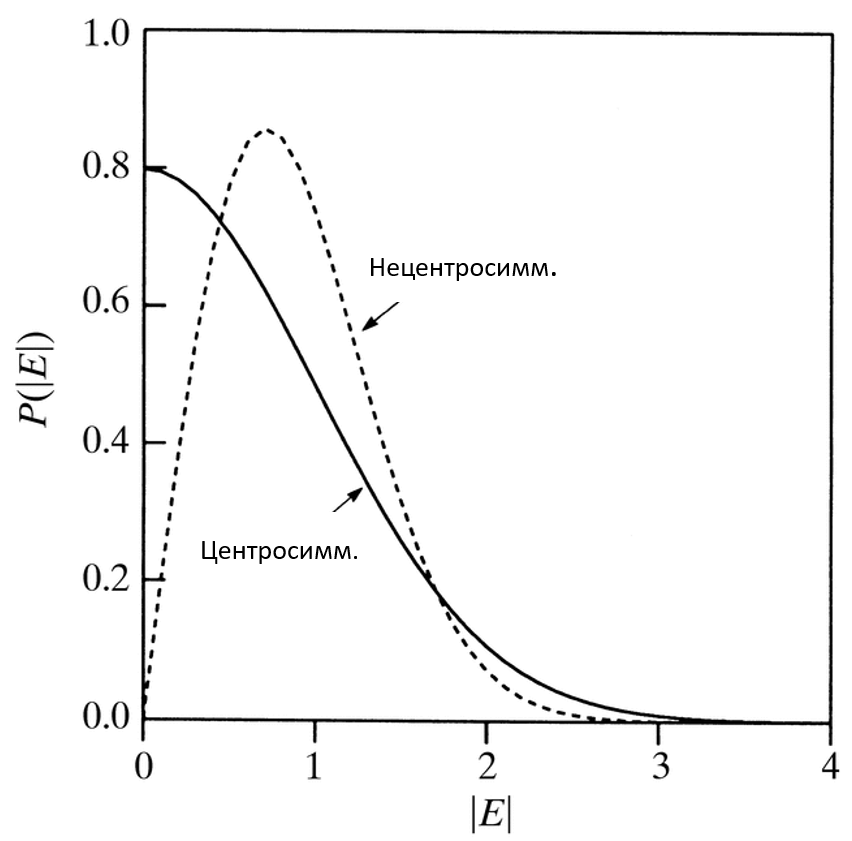
\includegraphics[width=0.5\textwidth]{figures/eimage.png}\hfill
	\caption{Плотность распределения $|E|$ для центросимметричных и нецентросимметричных кристаллов \cite{giacovazzo_international_2010}}
	\label{eimage}
\end{figure}

Прямые методы также основаны на структурных инвариантах~--- комбинации фаз рентгеновских отражений, сумма значений которых не меняется при сдвиге начала координат. Приведём некоторых из них. В работах \cite{sayre_squaring_1952}, \cite{cochran_relation_1952} была показана следующая взаимосвязь между высокоинтенсивными отражениями:

\begin{equation}\label{eq4}
\mathrm{ 
s(h+h', k+k', l+l') \approx s(h,k,l) s(h', k', l')}
\end{equation}


\begin{equation}\label{eq41}
\mathrm{
\phi(h+h', k+k', l+l')\approx \phi(h,k,l)+\phi(h',k',l')
}
\end{equation}

Из закона Фриделя следует, что:

\begin{equation}\label{eq5}
\mathrm{ 
\phi(-h-h',-k-k',-l-l') = -\phi(h+h', k+h', l+l')}
\end{equation}

Тогда, сложив уравнения \ref{eq5} и \ref{eq41} мы получим выражение, которое получило название триплетное отношение:

\begin{equation}\label{eq6}
\mathrm{ 
\phi(h,k,l)+\phi(h',k',l') +\phi(-h-h',-k-k',-l-l')\approx 0}
\end{equation}

Из данного уравнения и закона Фриделя так же нетрудно получить выражение для квартета отражений:

\begin{equation}\label{eq7}
\mathrm{ 
\phi(h,k,l)+\phi(h',k',l') +\phi(h'',k'',l'')+\phi(-h-h'-h'',-k-k'-k'',-l-l'-l'')\approx 0}
\end{equation}

Также нельзя не упомянуть важное равенство, которое является ключевым для прямых методов, а также нашло применение в других способах решения фазовой проблемы~--- формулу тангенсов, которая позволяет рассчитать фазу отражения \cite{karle_symbolic_1966}: 
 
 \begin{equation}\label{sigma2}
 	\mathrm{\tan\phi(\overrightarrow{H}) = \frac{\sum\limits_{\overrightarrow{K}}|E(\overrightarrow{K})E(\overrightarrow{H}-\overrightarrow{K})|\sin(\phi(\overrightarrow{K})+\phi(\overrightarrow{H}-\overrightarrow{K}))}{\sum\limits_{\overrightarrow{K}}|E(\overrightarrow{K})E(\overrightarrow{H}-\overrightarrow{K})|\cos(\phi(\overrightarrow{K})+\phi(\overrightarrow{H}-\overrightarrow{K}))}
 	}
 \end{equation}

На сегодняшний день прямые методы являются одним из наиболее используемых и популярных подходов для решения проблемы фаз в рентгеновской кристаллографии, незаменимыми для исследования малых и средних молекул. Основываясь на анализе статистических соотношений между нормализованными структурными факторами, эти методы позволяют оценить вероятные значения фаз с помощью структурных инвариантов, что делает возможным восстановление электронной плотности без дополнительных экспериментальных данных. Подробности расчётов и имплементации метода достаточно громоздки и достойны отдельного изучения \cite{giacovazzo_direct_1998}.

Прямые методы непрерывно совершенствуются: современные алгоритмы интегрируют классическую формулу тангенсов для оценки фаз с передовыми техниками модификации электронной плотности \cite{burla_robust_2013}. Такой гибридный подход позволяет не только получить более надёжные фазы благодаря доказанной статистической основе формулы тангенсов, но и существенно повысить качество и скорость сходимости решения за счёт итеративного улучшения электронной плотности в прямом пространстве. В результате объединения этих подходов удаётся достичь значительного повышения эффективности и надёжности решения проблемы фаз даже для сложных кристаллических структур.

\subsubsection{Метод Паттерсона}

Функция Паттерсона $P(\overrightarrow{u})$ представляет собой автокорреляционную функцию (свёртку функции с собой) электронной плотности \cite{girolami_x-ray_2016}:

\begin{equation}
	\mathrm{P(\overrightarrow{u}) = \int_V \rho(\overrightarrow{r})\rho(\overrightarrow{r}+\overrightarrow{u})d\overrightarrow{r}},
\end{equation}

где $\overrightarrow{u}$ --- вектор координат ячейки Паттерсона, которая совпадает по размерам с обычной, $V$ --- объем кристаллической решетки в прямом пространстве.

Из свойств автокорреляционной функции прямо следует, что функция Паттерсона $P(\overrightarrow{u})$ принимает ненулевые значения тогда и только тогда, когда электронная плотность принимает ненулевое значения в точке $\overrightarrow{r} = (x,y,z)$ и точке $\overrightarrow{r}+\overrightarrow{u} = (x+u, y+v, z+w)$, то есть в этих точках расположены атомы. Пики функции Паттерсона достигаются в таких точках, которые отвечает межатомным векторам кристалла.

Из экспериментальных данных функция Паттерсона рассчитывается следующим образом:

\begin{equation}\label{patt_start}
	\mathrm{P(\overrightarrow{u})=\frac{1}{V}}\sum_{\overrightarrow{H}}|F|^2(\overrightarrow{H})\exp(-2\pi i (\overrightarrow{H}, \overrightarrow{u}))
\end{equation}


Также можно выделить следующие свойства функции Паттерсона:

\begin{itemize}
	\item Функция Паттерсона всегда чётная, поскольку для каждой пары атомов существует пара межатомных векторов: $P(\overrightarrow{u}) = P(\overrightarrow{-u})$.
	\item Карта Паттерсона (графическое представление функции) обладает той же симметрией, что и группа Лауэ кристалла.
	\item Карта Паттерсона всегда имеет большой пик в начале координат --- явно следует из определения.
	\item Максимумы функции широкие и размазанные из-за перекрывания электронной плотности атомов.
\end{itemize}

Проанализируем количество максимумов функции Паттерсона \cite{rossmann_patterson_2001}. Пусть в элементарной ячейке $N$ атомов с атомными факторами рассеяния $f_j$. Из определения структурного фактора (уравнение \ref{eq1}) можно получить следующее выражение для $|F|^2$:

\begin{equation}
	\mathrm{|F(\overrightarrow{H})|^2 = F(\overrightarrow{H})F^*(\overrightarrow{H}) = \left[\sum\limits_{j=1}^N f_j \exp(2\pi i (\overrightarrow{H}, \overrightarrow{r_j}))\right]\left[\sum\limits_{j=1}^N f_j \exp(-2\pi i (\overrightarrow{H}, \overrightarrow{r_j}))\right]}
\end{equation}

\begin{equation}\label{patt1}
	\mathrm{|F(\overrightarrow{H})|^2 = \sum\limits_{j=1}^N f_j^2 + \sum\limits_{j=1}^N\sum\limits_{i=1, i\neq j}^N f_if_j\exp(2\pi i (\overrightarrow{H}, \overrightarrow{r_j}-\overrightarrow{r_i}))}
\end{equation}

Таким образом, объединив уравнения \ref{patt1} и \ref{patt_start}, получаем, что функция Паттерсона является суммой $N^2$ межатомных взаимодействий, из которых $N$ в начале координат с весами $f_j^2$ и $N(N-1)$ попарных взаимодействий, пропорциональных $f_if_j$. Таким образом, в карте Паттерсона $N(N-1)$ максимумов, которые зависят от межатомных векторов и типов атомов в ячейке. Нетрудно показать, что интенсивность этих пиков пропорциональна атомным номерам соответствующих атомов $Z_i$ (уравнение \ref{patt_z}, $m$~--- фактор мультиплетности). Поскольку функция Паттерсона является четной, для описания уникальных попарных взаимодействий достаточно $N(N-1)/2$ значений, поэтому часто используемым для представления данных является верхнетреугольная матрица. 

\begin{equation}\label{patt_z}
	\mathrm{P(\overrightarrow{u_{ij}}) = \frac{mZ_iZ_j}{\sum\limits_{j=1}^N f_j^2} }
\end{equation}

Поскольку $N$ максимумов карты Паттерсона, отвечающим свёртке электронной плотности каждого атома с самим собой, являются не очень информативными, от них можно избавиться, изменив структурные факторы перед расчётом функции Паттерсона по уравнению \ref{patt_mod_1}. Аналогично, если положения каких-то атомов заранее точно известны, пики, отвечающим их межатомным векторам, можно убрать благодаря модификации $|F(\overrightarrow{H})|^2$ в уравнении \ref{patt_mod_2}, где $r_1, r_2$ --- позиции известных атомов 1 и 2, $\sigma_1, \sigma_2$ --- их коэффициенты теплового движения.

\begin{equation}\label{patt_mod_1}
	\mathrm{|F_{mod}(\overrightarrow{H})|^2 = |F(\overrightarrow{H})|^2 - \sum\limits_{j=1}^Nf_j^2}
\end{equation}

\begin{equation}\label{patt_mod_2}
	\mathrm{|F_{mod}(\overrightarrow{H})|^2 = |F(\overrightarrow{H})|^2 - \sum\limits_{j=1}^Nf_j^2\sigma_j^2-2f_1f_2\sigma_1\sigma_2\cos(2\pi (\overrightarrow{H},\overrightarrow{r_1}-\overrightarrow{r_2}))}
\end{equation}

Для борьбы с шириной пиков, которые могут сильно повлиять на корректность определения фаз дифракционных отражений, используют процедуру сужение карты Паттерсона. Для этого вместо структурных факторов и их интенсивностей $|F|^2$ используют нормализованные структурные факторы $|E|^2$. Поскольку интенсивность нормализованных структурных факторов не так сильно падает с увеличением угла отражения $\theta$ благодаря поправочному множителю, полученный набор получен как бы от атомов меньшего размера, в результате чего максимумы Паттерсона также будут более узкие.

Карту Паттерсона можно представить суммой нескольких копий исходной структуры с разными весами \cite{buerger_solution_1953}, которые различаются тем, какой атом находится в начале паттерсоновских координат $(u, v, w)$ (рис. \ref{patterson_image}). Для простых структур низкомолекулярных соединений возможно расшифровать карту, сопоставив каждому максимуму межатомный вектор. Однако количество пиков функции Паттерсона для структуры из $N$ атомов растёт по квадратичному закону, что делает невозможным прямую интерпретацию без дополнительных операций над картой.

\begin{figure}[H]
	\centering
	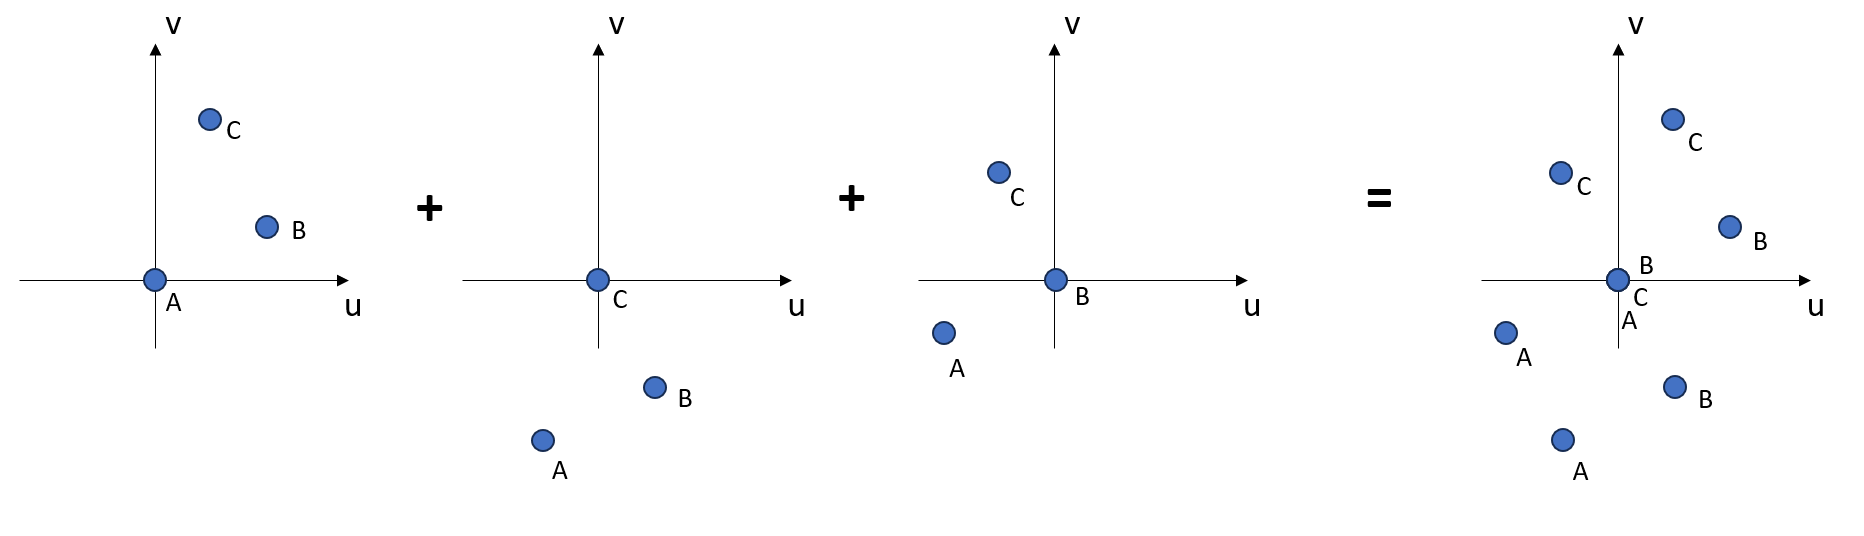
\includegraphics[width=1\textwidth]{figures/patterson.png}\hfill
	\caption{Схема карты Паттерсона для простейшей структуры из 3 атомов}
	\label{patterson_image}
\end{figure}

С развитием компьютерных технологий во второй половине 20 века произошел расцвет методов, основанных на функции Паттерсона. Так, особенно полезным для решения фазовой проблемы оказался метод суперпозиции карт Паттерсона \cite{hendrixson_locating_1997}. Было показано, что суперпозиция исходной карты Паттерсона со смещенной на какой-то трансляционный вектор может привести к меньшему набору межатомных векторов (рис. \ref{patt_superposition}), поскольку точки, соответствующие образу исходной структуры, будут всегда повторяться. Суперпозиция представляет собой, например, пересечение или сумму наборов векторов (см. далее). Через множество применений данной процедуры можно получить исходную структуру.

\begin{figure}[H]
	\centering
	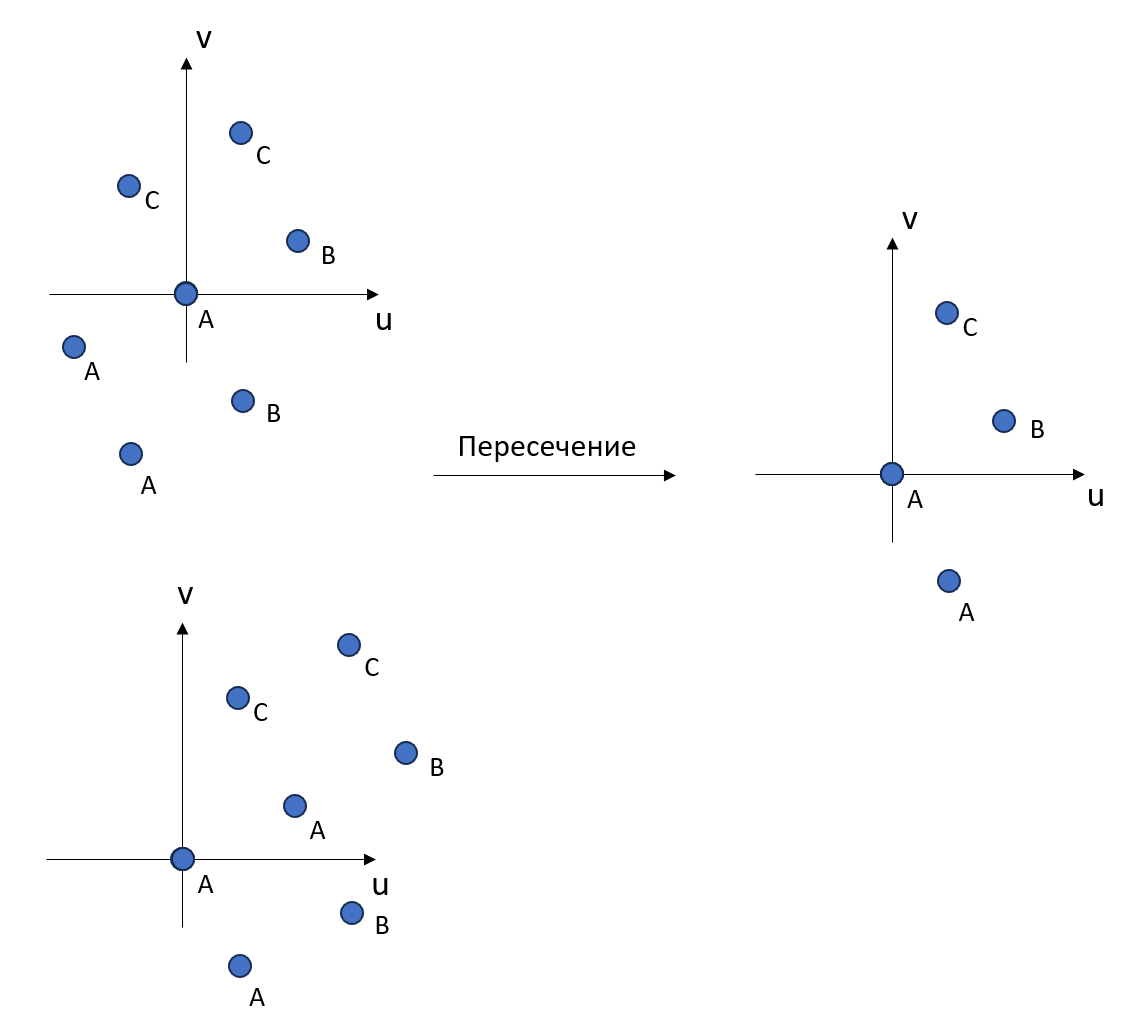
\includegraphics[width=0.8\textwidth]{figures/patt_superposition.png}\hfill
	\caption{Суперпозиция (пересечение) исходной и смещенной на вектор $\overrightarrow{AB}$ карт Паттерсона}
	\label{patt_superposition}
\end{figure}

Есть три основных подхода, которые используются для выделения структуры молекулы из наложенных карт Паттерсона --- с помощью функций суммы, произведения и минимума суперпозиции \cite{rossmann_patterson_2001}. Пусть есть $N$ карт Паттерсона, каждая из которых смещена на вектор $\overrightarrow{u_i}$. Функция суммы (уравнение \ref{patt_sum}) основывается на том, что она будет иметь наибольшие значения в точках пересечения всех карт, что будет отвечать расположениям атомов.

\begin{equation}\label{patt_sum}
	\mathrm{S(\overrightarrow{r}) = \sum\limits_{i=1}^N P(\overrightarrow{r}+\overrightarrow{u_i}) = \sum_{\overrightarrow{H}}}\left[|F(\overrightarrow{H})|^2 \exp (2\pi i (\overrightarrow{H}, \overrightarrow{r}))\left(\sum\limits_{j=1}^N\exp(2\pi i (\overrightarrow{H}, \overrightarrow{u_i}))\right)\right]
\end{equation}

Функция произведения суперпозиции (уравнение \ref{patt_prod}) является более сильной по сравнению с суммой в том смысле, что все точки, в которых нулевое значение хотя бы у одной из карт, будут обнулены.

\begin{equation}\label{patt_prod}
	\mathrm{Pr(\overrightarrow{r}) = \prod\limits_{i=1}^N P(\overrightarrow{r}+\overrightarrow{u_i})} 
\end{equation}
	
Если при наложении двух карт в точке ненулевая плотность, то суммарное значение функции Паттерсона будет больше, чем от одного изображения структуры. Если взять минимум от накладывающихся карт, то при удачной суперпозиции останется лишь плотность от одной копии структуры \cite{pavelcik_patterson-oriented_1992}. Так, в SHELXS-96 \cite{sheldrick_patterson_1997} имплементирован вариант суперпозиции карт Паттерсона с функцией минимума, которая берётся от двух копий утонченной функции Паттерсона, смещенных на векторы $\overrightarrow{u}$ и $\overrightarrow{-u}$.
	

\subsubsection{Метод обращенного заряда (charge--flipping)}

В работе \cite{oszlanyi_ab_2004} был предложен простой, но эффективный алгоритм --- метод обращенного заряда (charge--flipping), использующий свойства электронной плотности, а именно её неотрицательность. Данный алгоритм основан на итеративном приближении фаз дифракционных максимумов, которые в начале инициализируются случайными, к настоящим фазам, что позволяет решить фазовую проблему и определить кристаллическую структуру по дифракционным данным. 

Пусть в эксперименте был зарегистрирован набор дифракционных отражений, которые характеризуются амплитудами $F_{obs}(\overrightarrow{H})$. Незарегистрированные отражения в других точках обратного пространства принимаются за нулевые. Алгоритм начинается с инициализации фаз зарегистрированных отражений, которые выбираются случайным образом так, чтобы выполнялся закон Фриделя: $\phi(-\overrightarrow{H}) = -\phi(\overrightarrow{H})$. Получаем набор структурных факторов $F = F_{obs}(\overrightarrow{H})\exp(i\phi(\overrightarrow{H}))$.

Запишем основные шаги алгоритма:

\begin{enumerate}
	\item Для набора структурных факторов $F = F_{obs}(\overrightarrow{H})$ рассчитаем распределение электронной плотности $\rho(\overrightarrow{r})$, применив преобразование Фурье.
	\item Модифицируем электронную плотность $\rho(\overrightarrow{r})$ с помощью обращения заряда:
	
	\begin{equation}
		\mathrm{\rho(\overrightarrow{r})\geq \delta: g = \rho,}
	\end{equation}
	
	\begin{equation}
	\mathrm{\rho(\overrightarrow{r})<\delta: g = -\rho,}
	\end{equation}
		
	где $\delta > 0$ --- пороговое значение, параметр алгоритма.
	\item Переходим в обратное пространство, применив обратное преобразование Фурье к модифицированной электронной плотности $g(\overrightarrow{r})$. Получаем набор структурных факторов $G(\overrightarrow{H}) = |G(\overrightarrow{H})|\exp(i\psi(\overrightarrow{H}))$.
	\item Последнее преобразование называется ремодуляция. Собираем новый набор структурных факторов $F$ следующим образом: $F = F_{obs}(\overrightarrow{H})\exp(i\psi(\overrightarrow{H}))$ --- амплитуды равняются экспериментальным, фазы берутся из набора $G$, полученного в ходе обращения заряда. Вернуться к шагу 1.
\end{enumerate}

\begin{figure}[H]
	\centering
	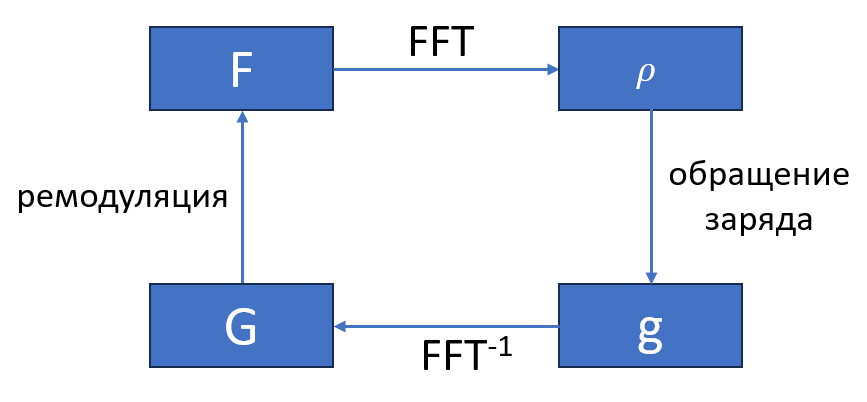
\includegraphics[width=0.8\textwidth]{figures/charge-flip.png}\hfill
	\caption{Схема итеративного цикла алгоритма charge--flipping}
	\label{chfl}
\end{figure}

В итерационный процесс (рис. \ref{chfl}) не заложено условие окончания алгоритма, для мониторинга процесса можно следить за метриками, такими как фактор расходимости R. Главными достоинствами метода являются его простота и отсутствие необходимости в дополнительных данных --- метод позволил получить структуры множества соединений $ab$ $initio$ при наличии лишь экспериментальных дифракционных данных высокого разрешения, задавая только пороговое значение $\delta$ для электронной плотности.

В следующей работе \cite{oszlanyi_it_2005} авторы модифицировали четвертый шаг метода, явно используя отражения низкой интенсивности. Перед запуском алгоритма дифракционные максимумы сортируются по наблюдаемой амплитуде и размечаются на две группы~--- сильные и слабые отражения, к которым будут применяться разные преобразования в ходе вычислений. Для сильных всё остается без изменений --- фазу берут из шага 2, амплитуда структурного фактора равняется экспериментальной. Фаза слабых отражений дополнительно смещается на $\Delta\phi$, а их амплитуда не изменяется на наблюдаемую. Это значит, что экспериментальные данные слабых отражений не используются в алгоритме, кроме начальной разметки на группы.

В модифицированном алгоритме charge--flipping появилось два дополнительных параметра: сдвиг фазы $\Delta\phi$ и доля отражений, которые можно считать слабыми, принятая за 20\%. Авторы показали, что оптимальное значение $\Delta\phi = \frac{\pi}{2}$ --- поскольку при сдвиге на такую величину волна слабого отражения становится ортогональной изначальной. Такое возмущение волн распространения низкоинтенсивных максимумов позволило на порядок увеличить долю успешных решений структур по сравнению с начальным алгоритмом.

Описанная модификация происходит в обратном пространстве, и в работе \cite{oszlanyi_charge_2008} авторы описывают подход к улучшению алгоритма с помощью изменения процедуры обработки функции электронной плотности. Charge--flipping в его классическом варианте можно рассматривать как алгоритм локального возмущения низких плотностей, то есть он никак не влияет на области с высокими значениями электронной плотности. Если в начале выполнения расчета будут получены некорректные высокие значения электронной плотности, то их практически невозможно исправить тривиальным обращением знака. В качестве аналога использования слабых отражений предлагается следующее улучшение в прямом пространстве (уравнения \ref{ccf1}, \ref{ccf2}).  Суть операции в следующем: измененная электронная плотность $g^{n+1}$ в $(n+1)$--й цикл алгоритма будет вне интервала, сформированными $\rho^{n-1}, \rho^{n}$, причем она будет ближе к $\rho^n$. Процедура получила название 'flip--mem' и значительно улучшает классический алгоритм.


\begin{equation}\label{ccf1}
	\mathrm{\rho^n(\overrightarrow{r}) < \delta: g^{n+1}(\overrightarrow{r}) = -\rho^n(\overrightarrow{r})},
\end{equation}
 
 
\begin{equation}\label{ccf2}
	\mathrm{\rho^n(\overrightarrow{r}) \geq \delta: g^{n+1} = \rho^n + \beta(\rho^n-\rho^{n-1})},
\end{equation} 
  
где обычно $\beta\in[0.5,1.0]$.

В этой же работе отмечено, что использование нормализованных структурных факторов $E(\overrightarrow{H})$ (уравнение \ref{e}) вместо стандартных амплитуд позволяет увеличить скорость сходимости для больших структур. Кроме того, все модификации, которые были ранее упомянуты, подходят и для варианта с нормализованными амплитудами. Использование $E(\overrightarrow{H})$ уменьшает на порядок число итераций до сходимости по сравнению с $F(\overrightarrow{H})$ для всех вариантов алгоритма.

Метод обращенного заряда позволяет в некоторых случаях решать макромолекулярные структуры $ab$ $initio$ \cite{dumas_macromolecular_2008}. Так, для таких структур, как лизоцим (2385 атомов, $d_{min} = 1.1 \text{\AA}$), алкогольдегидрогеназа(5866 атомов, $d_{min} = 1.0 \text{\AA}$), апамин (385 атомов, $d_{min} = 0.95 \text{\AA}$), фазы, рассчитанные алгоритмом, позволили корректно определить структуру. Авторы использовали метод в варианте с нормализованными структурными факторами $E(\overrightarrow{H})$, использованием слабых отражений (доля слабых отражений $\omega = 0.1$). Также авторы продемонстрировали, что charge--flipping является эффективным инструментов для нахождения фаз для рентгенодифракционных данных низкого разрешения сложных структур с тяжелыми атомами, а также с значимым анормальным рассеянием.

В работе \cite{coelho_charge-flipping_2007} авторы представили свой вариант алгоритма обращенного заряда с использованием нормализованных структурных факторов и новым способом возмущения, который применяет знание о формуле тангенсов, связывающей три отражения:

\begin{equation}\label{sigma3}
	\mathrm{\tan\phi_{tf}(\overrightarrow{H}) = \frac{\sum\limits_{\overrightarrow{K}}|E(\overrightarrow{K})E(\overrightarrow{H})E(\overrightarrow{H}-\overrightarrow{K})|\sin(\phi(\overrightarrow{K})+\phi(\overrightarrow{H}-\overrightarrow{K}))}{\sum\limits_{\overrightarrow{K}}|E(\overrightarrow{K})E(\overrightarrow{H})E(\overrightarrow{H}-\overrightarrow{K})|\cos(\phi(\overrightarrow{K})+\phi(\overrightarrow{H}-\overrightarrow{K}))}
	}
\end{equation}

Итоговый алгоритм (после случайной расстановки фаз для зарегистрированных отражений) выглядит следующим образом:

\begin{enumerate}
	\item Обнулить 50\% структурных факторов $E(\overrightarrow{H})$ с самыми низкими значениями амплитуд. Модуль остальных структурных факторов равен наблюдаемым.
	\item Рассчитать электронную плотность $\rho(\overrightarrow{r})$ с помощью обратного преобразования Фурье.
	\item Определить граничное значение $\delta$ так, что 60\% значений $\rho(\overrightarrow{r})$ лежат ниже порога.
	\item Преобразовать плотность:
	
	\begin{equation}
		\mathrm{\rho<\delta: g = -\rho}
	\end{equation}
	 
	\begin{equation}
		\mathrm{\rho\geq\delta: g = \delta + (\rho-\delta)^{1/2}}
	\end{equation}

	\item Рассчитать набор структурных факторов $G$, применив преобразование Фурье к электронной плотности $g(\overrightarrow{r})$
	\item Добавить к фазам с наибольшими значениями $E(\overrightarrow{H})$ долю разницы между фазами, полученной обратным зарядом $\phi_{cf}$ и рассчитанной по формуле тангенсов $\phi_{tf}$:
	
	\begin{equation}
		\mathrm{\phi(\overrightarrow{H}) = \phi_{cf}(\overrightarrow{H})+\alpha(\overrightarrow{H})(\phi_{tf}(\overrightarrow{H})-\phi_{cf}(\overrightarrow{H})),}
	\end{equation}
	 
	 где $\alpha(\overrightarrow{H})$ --- параметр, рассчитываемый алгоритмом для каждого отражения, который отражает достоверность рассчитанных в ходе выполнения программы фаз. Вернуться к шагу 1.
\end{enumerate}

Авторы продемонстрировали, что предложенный вариант метода позволяет решать за несколько минут структуры, которые ранее требовали сотни тысяч итераций. Использование формулы тангенсов для высокоинтенсивных отражений позволило повысить устойчивость и эффективность алгоритма, особенно при работе с низким разрешением данных (более $d_{min} = 1 \text{\AA}$), где классический вариант алгоритма чаще всего терпит неудачу.

В работе \cite{van_der_lee_charge_nodate} был проведен сравнительный анализ метода обращенного заряда с другими стандартными инструментами рутинного определения кристаллографических структур низкомолекулярных соединений. Для этого автор использовал charge--flipping в реализации программы SUPERFLIP \cite{palatinus_it_2007} и традиционные прямые методы --- SHELXS, SHELX86, SHELXD, SIR2004 \cite{sheldrick_shelxt_2015}. Тестирование проводилось на наборе данных из 518 структур, включащих в себя органические, металлорганические и неорганические соединения. Метод обращенного заряда показал эффективность, сравнимую с прямыми методами, в среднем процент успешного решения структур составляет более 92\%. На рис. \ref{charge_direct} представлены значения среднего R--фактора, достигаемого в ходе уточнения после успешного решения структур каждым методом. Также в статье показано, что charge--flipping является самым быстрым методом из рассматриваемых при той же эффективности решения. Таким образом, рассматриваемый алгоритм является полностью пригодным для определения низкомолекулярных структур в качестве рутинного метода.


\begin{figure}[H]
	\centering
	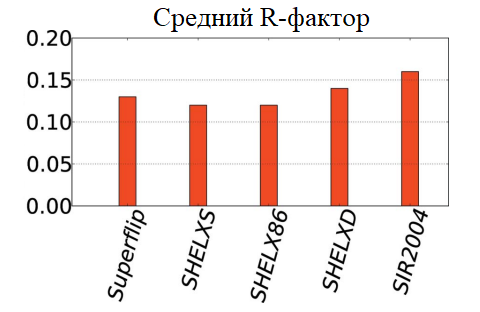
\includegraphics[width=0.5\textwidth]{figures/charge_direct.png}\hfill
	\caption{Средний R--фактор успешных решений различных методов решения}
	\label{charge_direct}
\end{figure}

\subsubsection{Метод Vive La Diff\'erence (VLD)}

Следующий рассматриваемый метод под названием Vive La Diff\'erence (VLD) является эффективным и универсальным методом для определения кристаллических структур, основанным на преобразовании электронной плотности и разностном Фурье--синтезе исходя из вероятностных и статических зависимостей между фазами и амплитудами \cite{burla_random_2010}. Как и charge--flipping, метод является итеративным, но более комплексным, чем метод обращенного заряда. Перед стартом расчёта фаз всем наблюдаемым амплитудам нормализованных структурных факторов $E_{obs}$ присваиваются случайные фазы $\phi_m$ и рассчитывается электронная плотность кристаллической ячейки $\rho_m$. Здесь и далее величины, определяемые в ходе выполнения расчёта, назовём модельными. Алгоритм состоит из следующих шагов (схема представлена на рис. \ref{vld}):

\begin{enumerate}
	\item Модифицируем электронную плотность $\rho(\overrightarrow{r})$ следующим образом: обнуляем функцию во всех точках, кроме 2.5\% с наибольшим значением плотности. По полученной измененной электронной плотности $g(\overrightarrow{r})$ рассчитываем модельные нормализованные структурные факторы $E_m$ с помощью Фурье--преобразования.
	\item Вычисляем разностную электронную плотность --- синтез Фурье со следующими коэффициентами для каждого отражения:
	
	\begin{equation}
		\mathrm{\Delta E = (mE_{obs} - E_m)\exp(i\phi_m)}
	\end{equation}
		
	где $m$ --- коэффициент корреляции между модельными и реальными фазами.
	
	\item Модифицируем полученную разностную плотность: обнуляем функцию во всех точках, кроме 4\% с наибольшим значением по модулю. С помощью Фурье--преобразования рассчитываем разностные структурные факторы с амплитудами и фазами $E_{diff}, \phi_{diff}$.
	
	\item Используем полученные из разностной электронной плотности структурные факторы для расчёта коэффициента Фурье--синтеза (шаг 2), рассчитываем новую разностную плотность. Повторяем настоящий и предыдущий шаги $\beta$ раз, итоговые параметры структурных факторов $E_{diff}', \phi_{diff}'$.
	
	\item С помощью формулы тангенсов, которая была получена из вероятностного анализа и распределения фон Мизеса, можно рассчитать новые фазы $\phi_{calc}$:
	
	\begin{equation}
		\mathrm{\tan(\theta) = \frac{E_m\sin\phi_m+\omega_{diff}E_{diff}\sin\phi_{diff}}{E_m\cos\phi_m+\omega_{diff}E_{diff}\cos\phi_{diff}}}
	\end{equation}
	
	где $\omega_m$ --- параметр сходства модельной и реальной структур, отражающий среднюю корреляцию между моделью и структурой.
	
	\item Экспериментальные $E_{obs}$ и рассчитанные на предыдущем шаге фазы $\phi_{calc}$ используются для расчета электронной плотности, которая претерпевает $\gamma$ циклов модификации, как в шаге 1. 
	
	\item Рассчитывается метрика $RESID$ --- средняя ошибка между наблюдаемыми и рассчитанными амплитудами:
	
	\begin{equation}
		\mathrm{RESID = \frac{\sum_{\overrightarrow{H}}|E_{obs} - E_m|}{\sum_{\overrightarrow{H}}E_{obs}}}
	\end{equation}

	Если значение меньше 0.3 --- можно считать, что решение достигнуто и цикл останавливается. Иначе --- возвращение к шагу 1.
\end{enumerate}


\begin{figure}[H]
	\centering
	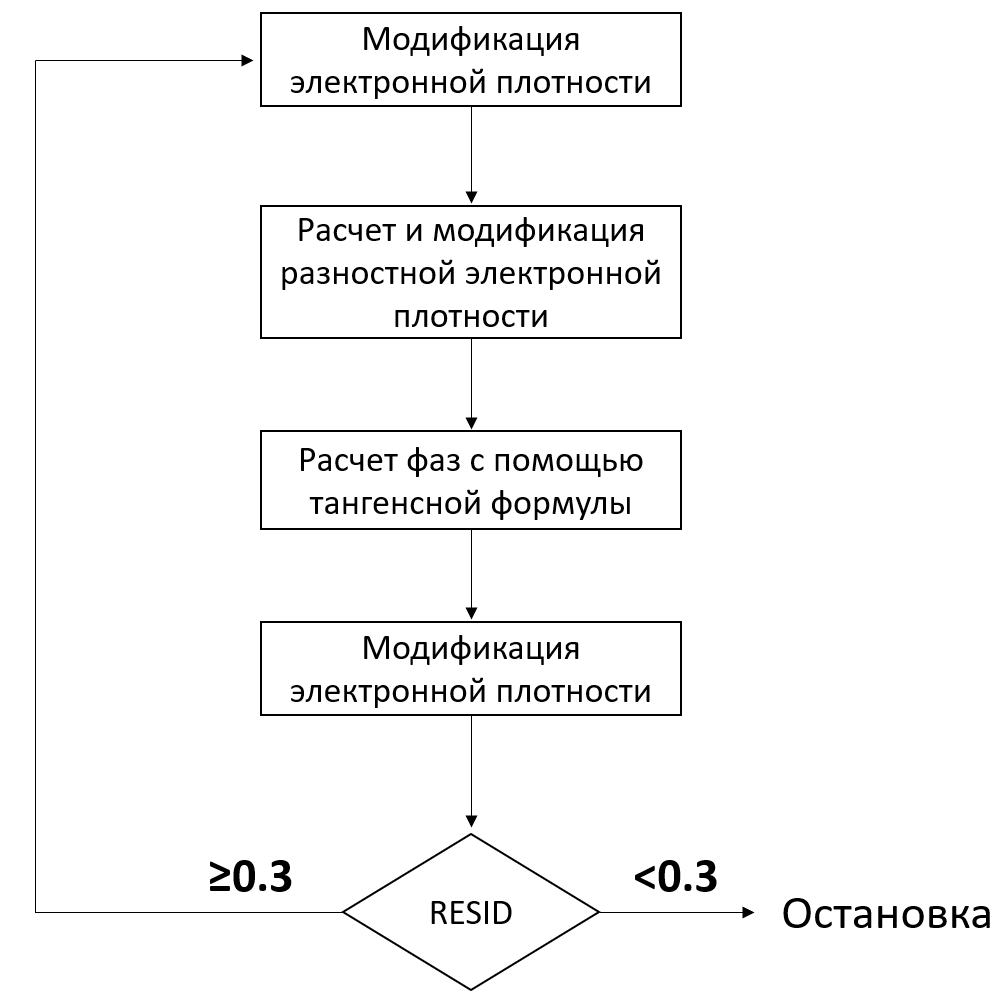
\includegraphics[width=0.7\textwidth]{figures/vld.png}\hfill
	\caption{Схема итеративного цикла алгоритма VLD}
	\label{vld}
\end{figure}

Подробности процедур выбора настраиваемых параметров алгоритма и рассчета критических параметров, как $\omega_m$ и $m$, подробно описаны в оригинальной работе. Авторы протестировали предложенный метод на 33 низкомолекулярных структурах, разных по пространственной группе симметрии и наличию тяжелых атомов, из которых VLD успешно решил 30 структур за не более, чем 300 циклов. При дополнительных запусках с другими случайными фазами при инициализации модели привели к решению всего набора данных. Таким образом, показано, что метод является достаточно стабильным и обладает быстрой сходимостью (менее, чем 1 минута). Важно отметить, что в отличие от метода обращенного заряда, метод решает структуру в правильной группе симметрии, а не P1.

В следующей работе \cite{burla_advances_2011} авторы развивают идеи первой работы и описывают существенные усовершенствования оригинального подхода к решению кристаллографической фазовой проблемы. Ключевым усовершенствованием является внедрение процедуры RELAX, которая позволяет автоматически переместить правильно ориентированную, но смещённую модель в корректное начальное положение в пространственной группе. RELAX основана на наблюдении, что прямые методы определяет молекулярные фрагменты, которые корректно ориентированы, но неправильно расположены. Использование процедуры существенно повысило процент успешно решённых структур, особенно в случае макромолекулярных соединений. Также в статье представлено значительное количество улучшений, связанные с улучшенной оценкой параметров качества модели, оптимизацией этапов модификаций электронной плотности, а также дополнительные параметры качества решений для управления остановкой VLD. Тестирование на малых, средних молекулах и белках (разрешение до $d_min = 1.2 \text{\AA}$) показало, что доработанный алгоритм решает структуры быстрее в среднем в 3--6 раз, определяет структуры белков за время, сравнимое с прямыми методами (SIR2011), а добавление RELAX позволило находить решения для крупных молекул именно благодаря этой процедуре.

В публикации \cite{burla_phasing_2011} представлено множество дополнительных вариантов алгоритма VLD (4 протокола), которые ориентированы на решение проблемы фаз для среднемолекулярных и белковых соединений. Вариации метода различаются подходами к контролю метрик сходимости и внутренних параметров, а также способами комбинирования модели, разностной и обычной электронных плотностей (количество преобразований Фурье, использование или игнорирование экспериментальных данных, а также отказ от формулы тангенсов). В ходе оценки эффективности показано, что новые подходы уступают по успешности и скорости решения варианту с процедурой RELAX, но могут быть в дальнейшем оптимизированы для $ab$ $initio$ решения макромолекулярных соединений.


\subsubsection{Методы искусственного интеллекта}

Применение методов машинного обучения в рентгенодифракционных исследованиях~--- область, демонстрирующая стремительное развитие. Традиционно анализ дифракционных данных и решение обратной задачи в кристаллографии базировались на строго детерминированных алгоритмах, использующих априорные физические и химические знания о структуре вещества. Однако с ростом объёмов экспериментальных данных, увеличением доступной вычислительной мощности и успехами в смежных областях — таких как обработка изображений, анализ временных рядов и предсказание структур белков — возник интерес к использованию ИИ как инструмента для автоматизации и улучшения интерпретации дифракционных данных.

Первая публикация с решением фазовой проблемы методами глубокого обучения была опубликована почти год назад \cite{larsen_phai_2024}. Для предсказания были выбраны центросимметричные структуры (группы симметрии $P2_1/c, C2/c, Pbca, Pnma, Pbcn, C2/m$), фазы дифракционных максимумов которых принимают два возможных значения~--- 0 и $\pi$ \cite{cowtan_phase_2003}. Для обучения авторы сгенерировали 49 млн. синтетических структур, подавляюющее большинство которых~--- органические и небольшая доля металлорганических. Нейронная сеть PhAI представляет собой бинарных классификатор из блоков трехмерных свёрток и многослойных перцептронов (рис. \ref{phai}). Также в архитектуре сети представлен рециклинг фаз~--- данные прогоняются несколько раз через модель, чтобы добиться лучшего качества определения фаз отражений. Нейронная сеть использует только амплитуды структурных факторов, и достигает сопоставимого качества решения с методом обращенного заряда. Нельзя не упомянуть, что модель способна решить фазовую проблему при разрешении рентгенодифракционных данных всего 2.0 \AA, то есть используя лишь 10--20\% объема данных, необходимых классическим методам. Авторы продемонстрировали высокую точность на экспериментальных данных, а также способность к предсказанию фаз для отсутствующих фаз (расширение фаз, phase extension). Таким образом, впервые был продемонстрирован потенциал машинного обучения для определения фаз. Недостатком модели является то, что она заточена под центросимметричные структуры. Исключительный интерес же представляют нецентросимметричные кристаллы, к которым нельзя будет применить подход с бинарным классификатором, описанным в работе.

\begin{figure}[H]
	\centering
	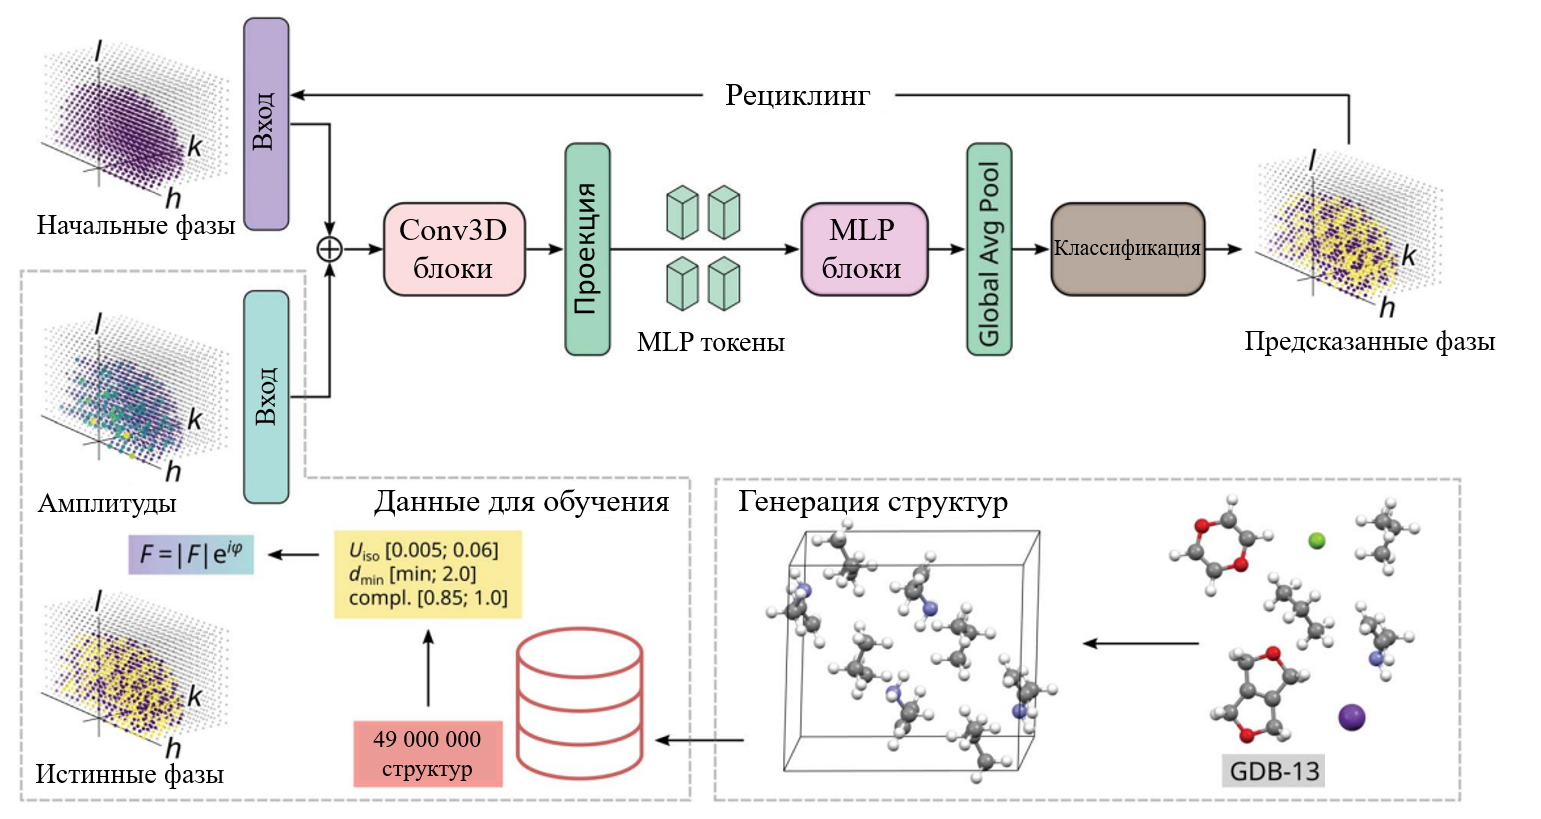
\includegraphics[width=1\textwidth]{figures/phai.png}\hfill
	\caption{Схема нейронной сети PhAI для решения проблемы фаз \cite{larsen_phai_2024}}
	\label{phai}
\end{figure}

Вдохновившись описанным исследованием, авторы \cite{carrozzini_phase-seeding_2025} предлагают адаптацию его идеи для нецентросимметричных структур. В работе предложен метод phase seeding, который позволяет переформулировать задачу из регрессионной с определением непрерывных величин от 0 до $2\pi$ в задачу мультиклассовой классификации. Сначала весь диапазон фаз дискретизируется в ограниченный набор промежутков, в каждом из которых фазы отражений заменяют на одинаковое значение (рис. \ref{phase_disc}). Затем фаза каждого отражения случайным образом относится к одному из подмножеств. Авторы продемонстрировали на различных структурах, что для решения структур детерминированными методами достаточно будет предсказать с помощью методов искусственного интеллекта одно из дискретных значений фаз для каждого дифракционного максимума. Также предложено для решения фазовой проблемы методами ИИ использовать отражения с наибольшими значениями амплитуды нормализованного структурного фактора $E$.

\begin{figure}[H]
	\centering
	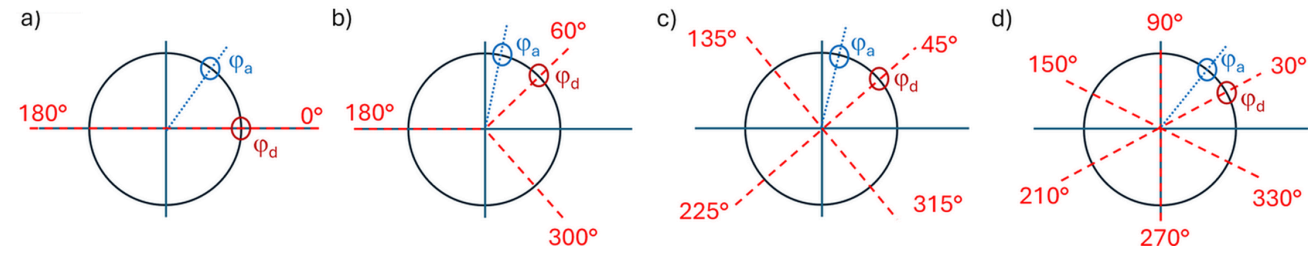
\includegraphics[width=1\textwidth]{figures/phase_disc.png}\hfill
	\caption{Дискретизация значений фаз: на 2 промежутка (а), на 3 промежутка (b), на 4 промежутка (c), на 6 промежутков (d). Истинное значение фазы~--- $\phi_a$ (синий круг), дискретизованное~--- $\phi_d$ (красный круг) \cite{carrozzini_phase-seeding_2025}}
	\label{phase_disc}
\end{figure}

Также были совершены попытки предсказать структуры белков напрямую из экспериментальных данных, минуя этап с определением фазовой информации. Так, была предложена модель RecCrysFormer, позволяющая напрямую предсказывать электронную плотность макромолекулярных соединений на основе карт Паттерсона и известной плотности отдельных белковых фрагментов \cite{pan_reccrysformer_2025}. Архитектура сети представляет собой трехмерные сверточные слои, переводящие карту Паттерсона и плотность в пространство признаков, которые затем подаются на вход в трансформер, выходные данные которого обрабатываются с помощью слоёв многослойного перцептрона и трехмерных свёрток для получения карт плотности всего белка. Примечательно, что в слое трансформера реализовано одностороннее внимание, поэтому только токены функции Паттерсона "смотрят" на токены фрагментов соединения. Авторы смогли добиться решения 93\% тестовых структур, хотя и признают, что выбранные ими соединения меньше реальных белков.

Были найдены решения фазовой проблемы с помощью методов глубокого обучения в области физики, а именно в рамках метода когерентной безлинзовой микроскопии \cite{wang_use_2024}. В обзорной статье выделены 3 подхода (рис. \ref{dl})~--- DL-pre-processing, в котором обученная модель повышает разрешение дифракционных данных, после чего проблема фаз решается классическими детерминированными методами; DL-in-processing, в рамках которого из экспериментальных интенсивности с помощью нейронной сети рассчитывают фазы напрямую; DL-post-processing, в котором уточняются зашумленные приближенные фазы, полученные из исходных интенсивностей. Несмотря на то, что для рентгеновской кристаллографии нельзя напрямую использовать уже готовые методы микроскопии, поскольку данные сильно различаются разрешением, эти идеи можно адаптировать. Так, существующее решение PhAI \cite{larsen_phai_2024} можно отнести к DL-in-processing.

\begin{figure}[H]
	\centering
	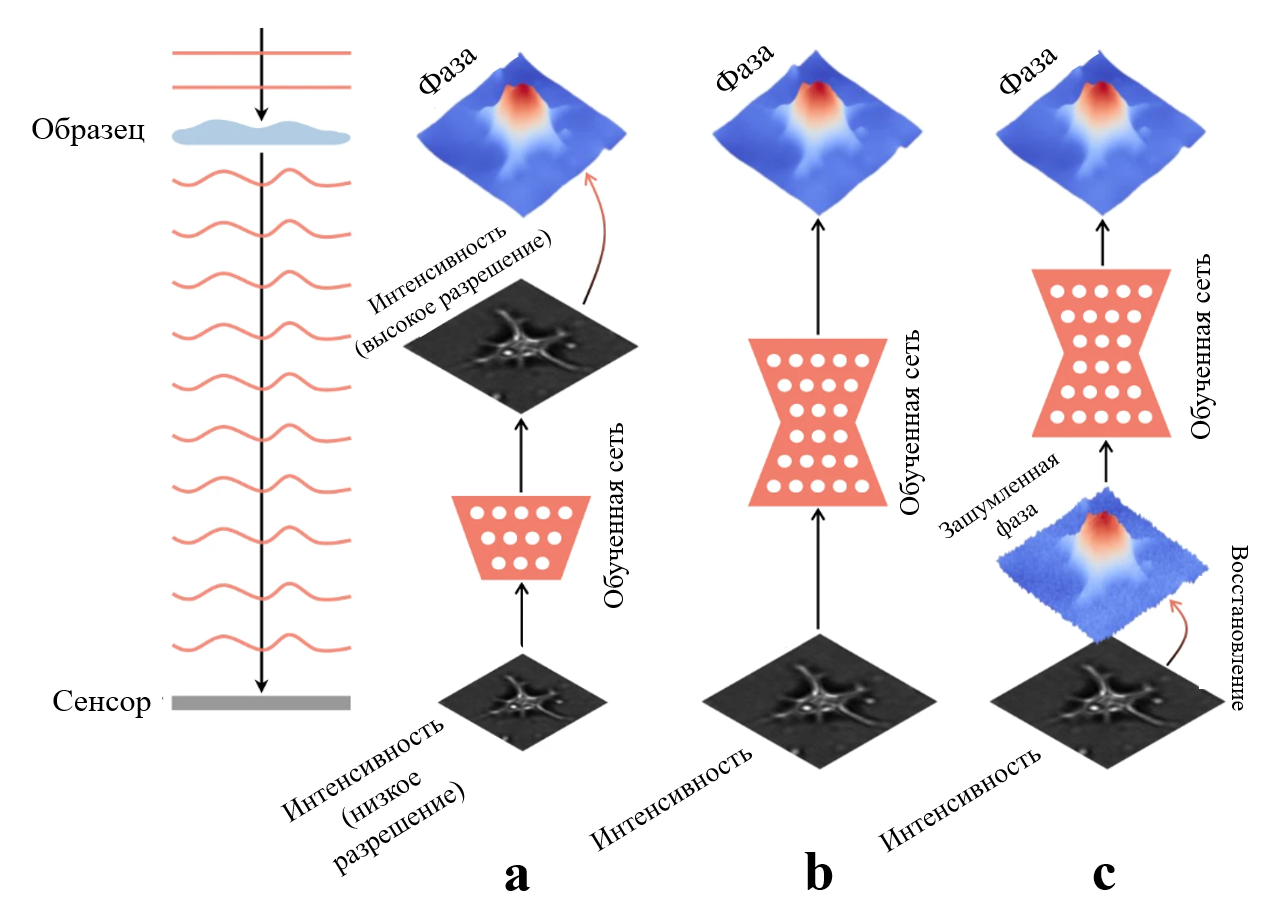
\includegraphics[width=1\textwidth]{figures/dl.png}\hfill
	\caption{Подходы к восстановлению фаз в микроскопии: DL-pre-processing (a), DL-in-processing (b), DL-post-processing (c) \cite{wang_use_2024}}
	\label{dl}
\end{figure}

\subsection{Заключение}

Проблема фаз является фундаментальной задачей рентгенодифракционных исследований кристаллов, без решения которой невозможно определить структуру кристалла. На сегодняшний день существует множество методов, позволяющих преодолеть отсутствие информации о фазах дифракционных максимумов, но они имеют ряд ограничений, связанных с требованием к достаточно высокому разрешению данных. Данное требование может не выполняться в рамках белковой кристаллографии, где фазовая проблема исключительно редко решается рутинными методами. Для определения структур макромолекулярных соединений требуется дополнительная информацая — знание о структуре белка с той же аминокислотной последовательностью или результаты рентгенодифракционных экспериментов той же структуры с добавлением тяжелых атомов. Поэтому решение проблемы фаз является особенно актуальной задачей для исследователей белковых структур.

Однако инструменты на основе методов глубокого обучения способны преодолеть ограничения традиционных подходов, поскольку уже продемонстрирован их потенциал к определению кристаллических структур на основе ограниченных рентгенодифракционных данных с низким разрешением. По мере развития исследований в этой области, вероятно, алгоритмы искусственного интеллекта станут незаменимым инструментом в области кристаллографии, облегчая решение сложных структур.

Таким образом, целью данной работы является разработка и исследование применимости методов искусственного интеллекта для решения проблемы фаз.

В рамках данной цели были выделены следующие задачи:

\begin{enumerate}
	\item Разработать программное обеспечение, позволяющее создать набор синтетических рентгенодифракционных данных для обучения нейронных сетей;
	\item Разработать программное обеспечение, с помощью которого можно проводить воспроизводимые численные эксперименты по обучению и тестированию моделей;
	\item Разработать и обучить подходящие модели глубокого обучения;
	\item Произвести анализ полученных моделей на эффективность решения фазовой проблемы для реальных структур.
\end{enumerate}